\chapter{The Heat Equation}\label{chap1}

LET\pageoriginale US CONSIDER the equation
\begin{equation*}
u_{t}-\frac{1}{2}\Delta u=0\tag{1}\label{chap1-eq1}
\end{equation*}
which describes (in a suitable system of units) the temperature
distribution of a certain homogeneous, isotropic body in the absence
of any heat sources within the body. Here
$$
u\equiv u(x_{1},\ldots,x_{d},t);\quad u_{t}\equiv \frac{\p u}{\p
  t};\quad \Delta u=\sum^{d}_{i=1}\frac{\p^{2}u}{\p x^{2}_{i}},
$$
$t$ represents the time ranging over $[0,\infty)$ or $[0,T]$ and
  $x\equiv (x_{1}\ldots x_{d})$ belongs to $\mathbb{R}^{d}$. 

We first consider the initial value problem. It consists in
integrating equation \eqref{chap1-eq1} subject to the initial
condition
\begin{equation*}
u(0,x)=f(x).\tag{2}\label{chap1-eq2}
\end{equation*}

The relation \eqref{chap1-eq2} is to be understood in the sense that 
$$
{\displaystyle{\mathop{\text{Lt}}_{t\to 0}}}u(t,x)=f(x).
$$

Physically \eqref{chap1-eq2} means that the distribution of
temperature throughout the body is known at the initial moment of
time.

We assume that the solution $u$ has continuous derivatives, in the
space coordinates upto second order inclusive and first order
derivative in time.

It is easily verified that
\begin{equation*}
u(t,x)=\frac{1}{(2\pi t)^{d/2}}\exp
\left(-\frac{|x|^{2}}{2t}\right);\quad |x|^{2}=\sum^{d}_{i=1}x^{2}_{i},\tag{3}\label{chap1-eq3}
\end{equation*}
satisfies\pageoriginale \eqref{chap1-eq1} and
\begin{equation*}
u(0,x)=\Lt\limits_{t\to 0} u(t,x)=\delta (x)\tag{4}\label{chap1-eq4}
\end{equation*}

Equation \eqref{chap1-eq4} gives us a very nice physical
interpretation. The solution \eqref{chap1-eq3} can be interpreted as
the temperature distribution within the body due to a unit sourse of
head specified at $t=0$ at the space point $x=0$. The linearity of the
equation \eqref{chap1-eq1} now tells us that (by superposition) the
solution of the initial value problem may be expected in the form
\begin{equation*}
u(t,x)=\int\limits_{\mathbb{R}^{d}}f(y)p(t,x-y)dy,\tag{5}\label{chap1-eq5}
\end{equation*}
where
$$
p(t,x)=\frac{1}{(2\pi t)^{d/2}}\exp -\frac{|x|^{2}}{2t}.
$$

\begin{exercise}\label{chap1-exer1}
Let $f(x)$ be any bounded continuous function. Verify that $p(t,x)$
satisfies \eqref{chap1-eq1} and show that
\begin{itemize}
\item[(a)] $\int p(t,x)dx=1$, $\forall t>0$;

\item[(b)] $\Lt\limits_{t\to 0+}\int p(t,x)f(x)dx=f(0)$;

\item[(c)] using (b) justify \eqref{chap1-eq4}. Also show that
  \eqref{chap1-eq5} solves the initial value problem.
\end{itemize}
(Hints: For (a) use
$\int\limits^{\infty}_{-\infty}e^{-x^{2}}dx=\sqrt{\pi}$. For part (b)
make the substitution $y=\dfrac{x}{\sqrt{\pi}}$ and apply Lebesgue
dominated convergence theorem). 
\end{exercise}

Since equation \eqref{chap1-eq1} is linear with constant coefficients
it is invariant under time as well as space translations. This means
that translates of solutions are also solutions. Further, for $s\geq
0$,\pageoriginale $t>0$ and $y\in \mathbb{R}^{d}$,
\begin{equation*}
u(t,x)=\frac{1}{[2\pi(t+s)]^{d/2}}\exp-\frac{|x-y|^{2}}{2(t+s)}\tag{6}\label{chap1-eq6}
\end{equation*}
and for $t>s$, $y\in \mathbb{R}^{d}$,
\begin{equation*}
u(t,x)=\frac{1}{[2\pi(t-s)]^{d/2}}\exp-\frac{|x-y|^{2}}{2(t-s)}\tag{7}\label{chap1-eq7}
\end{equation*}
are also solutions of the heat equation \eqref{chap1-eq1}.

The above method of solving the initial value problem is a sort of
trial method, viz.\@ we pick out a solution and verify that it
satisfies \eqref{chap1-eq1}. But one may ask, how does one obtain the
solution? A partial clue to this is provided by the method of Fourier
transforms. We pretend as if our solution $u(t,x)$ is going to be very
well behaved and allow all operations performed on $u$ to be
legitimate.

Put $v(t,x)=\hat{u}(t,x)$ where $\sphat$ stands for the Fourier
transform in the space variables only (in this case), i.e.
$$
v(t,x)=\int\limits_{\mathbb{R}^{d}}u(t,y)e^{i\ x-y}dy.
$$

Using equation \eqref{chap1-eq1}, one easily verifies that
\begin{equation*}
v_{t}(t,x)=\frac{1}{2}|x|^{2}v(t,x)\tag{8}\label{chap1-eq8}
\end{equation*}
with 
\begin{equation*}
v(0,x)=\hat{f}(x).\tag{9}\label{chap1-eq9}
\end{equation*}

The solution of equation \eqref{chap1-eq8} is given by
\begin{equation*}
v(t,x)=\hat{f}(x)e^{-t|x|^{2}/2}.\tag{10}\label{chap1-eq10}
\end{equation*}

We have used \eqref{chap1-eq9} in obtaining \eqref{chap1-eq10}.

\begin{exercise}\label{chap1-exer2}
Verify\pageoriginale that 
$$
\hat{p}(t,x)=\exp -\left(\frac{t|x|^{2}}{2}\right).
$$
\end{exercise}

Using Exercise \ref{chap1-exer2}, \eqref{chap1-eq10} can be written as
\begin{equation*}
v(t,x)=\hat{u}(t,x)=\hat{f}(x)\hat{p}(t,x).\tag{11}\label{chap1-eq11}
\end{equation*}

The right hand side above is the product of two Fourier transforms and
we know that the Fourier transform of the convolution of two funtions
is given by the product of the Fourier transforms. Hence $u(t,x)$ is
expected to be of the form \eqref{chap1-eq5}.

Observe that if $f$ is non-negative, then $u$ is nonnegative and if
$f$ is bounded by $M$ then $u$ is also bounded by $M$ in view of part
(a) of Exercise \ref{chap1-exer1}.

\medskip
\noindent
{\bf The Inhomogeneous Equation.}~ Consider the equation
$$
v_{t}-\frac{\Delta v}{2}=g,\quad\text{with}\quad v(0,x)=0,
$$
which describes the temperature within a homogeneous isotropic body in
the presence of heat sources, specified as a function of time and
space by $g(t,x)$. For $t>s$,
$$
u(t,x)=\frac{1}{[2\pi(t-s)]^{d/2}}\exp -\frac{|x-y|^{2}}{2(t-s)}
$$
is a solution of $u_{t}(t,x)-\dfrac{1}{2}\Delta u(t,x)=0$
corresponding to a unit source at $t=s$, $x=y$. Consequently, a
solution of the inhomogeneous problem is obtained by superposition.

Let
$$
v(t,x)=\int\limits_{\mathbb{R}^{d}}\int\limits^{t}_{0}g(s,y)\frac{1}{[2\pi(t-s)]^{d/2}}\exp
\left(-\frac{|x-y|^{2}}{2(t-s)}\right)dy\ ds
$$
i.e.\pageoriginale
$$
v(t,x)=\int\limits^{t}_{0}w(t,x,s)ds
$$
where
$$
w(t,x,s)=\int\limits_{\mathbb{R}^{d}}g(s,y)\frac{1}{[2\pi(t,s)]^{d/2}}\exp\left(-\frac{|x-y|^{2}}{2(t-s)}\right)dy.
$$

\begin{exercise}\label{chap1-exer3}
Show that $v(t,x)$ defined above solves the inhomogeneous heat
equation and satisfies $v(0,x)=0$. Assume that $g$ is sufficiently
smooth and has compact support. $v_{t}-\dfrac{1}{2}\Delta
v=\Lt\limits_{s\to t}w(t,x,s)$ and now use part (b) of Exercise
\eqref{chap1-exer1}. 
\end{exercise}

\begin{remark}\label{chap1-rem1}
We can assume $g$ has compact support because in evaluating
$v_{t}-\dfrac{1}{2}\Delta v$ the contribution to the integral is
mainly from a small neighbourhood of the point $(t,x)$. Outside this
neighbourhood
$$
\frac{1}{[2\pi(t-s)]^{d/2}}\exp \left(-\frac{|x-y|^{2}}{2(t-s)}\right)
$$
satisfies
$$
u_{t}-\frac{1}{2}\Delta u=0.
$$

2.~ If we put $g(s,y)=0$ for $s<0$, we recognize that $v(t,x)=g\ast
p$. Taking spatial Fourier transforms this can be written as
$$
v(t,\xi)=\int\limits^{t}_{0}g(s,\xi)\exp
-\frac{1}{2}(t-s)|\xi|^{2}d\xi,
$$
or
$$
\frac{\p \hat{v}}{\p t}=\frac{\p v}{\p t}=g(t,\xi)+\frac{1}{2}\Delta
v=\left(g(t,\xi)+\frac{1}{2}\Delta v\right).
$$

Therefore
$$
\frac{\p v}{\p t}-\frac{1}{2}\Delta v=g.
$$
\end{remark}

\begin{exercise}\label{chap1-exer4}
Solve\pageoriginale $w_{t}-\dfrac{1}{2}\Delta w=g$ on
$[0,\infty)\times\mathbb{R}^{d}$ with $w=f$ on $\{0\}\times
  \mathbb{R}^{d}$ (Cauchy problem for the heat equation).
\end{exercise}

\smallskip
\noindent
{\bf Uniqueness.}~ The solution of the Cauchy problem is unique
provided the class of solutions is suitably restricted. The uniqueness
of the solution is a consequence of the Maximum Principle.

\medskip
\noindent
{\bf Maximum Principle.}~ {\em Let $u$ be smooth and bounded on
  $[0,T]\times\mathbb{R}^{d}$ satisfying}
$$
u_{t}-\frac{\Delta u}{2}\geq 0\quad\text{in}\quad
(0,T]\times\mathbb{R}^{d}\quad\text{and}\quad u(0,x)\geq 0,\ \forall
x \in \mathbb{R}^{d}. 
$$

{\em Then}
$$
u(t,x)\geq 0 \ \ \forall,\quad t\in [0,T]\quad\text{and}\quad \forall x
\in \mathbb{R}^{d}.
$$

\begin{proof}
The idea is to find minima for $u$ or for an auxillary function.


\begin{step}
Let $v$ be {\em any} function satisfying
$$
v_{t}-\frac{\Delta v}{2}>0\quad\text{in}\quad (0,T]\times
\mathbb{R}^{d}.
$$
\end{step}

\begin{claim*}
$v$ cannot attain a minimum for $t_{0}\in (0,T]$. Assume (to get a
contradiction) that $v(t_{0},x_{0})\leq v(t,x)$ for some $t_{0}>0$ and
for all $t\in [0,T]$, $\forall x\in \mathbb{R}^{d}$. At a minimum
$v_{t}(t_{0},x_{0})\leq 0$, (since $t_{0}\neq 0$) $\Delta
v(t_{0},x_{0})\geq 0$. Therefore
$$
\left(v_{t}-\frac{\Delta v}{2}\right)(t_{0},x_{0})\leq 0.
$$

Thus, if $v$ has any minimum it should occur at $t_{0}=0$.
\end{claim*}

\begin{step}
Let $\epsilon>0$ be arbitrary. Choose $\alpha$ such that
$$
h(t,x)=|x|^{2}+\alpha t
$$
satisfies\pageoriginale
$$
h_{t}-\frac{\Delta h}{2}=\alpha -d>0\quad(\text{say~ }\alpha =2d).
$$

Put $v_{\epsilon}=u+\epsilon h$. Then
$$
\frac{\p v_{\epsilon}}{\p t}-\frac{1}{2}\Delta v_{\epsilon}>0.
$$

As $u$ is bounded, $v_{\epsilon}\to +\infty$ as $|x|\to +\infty,\;
v_{\epsilon}$ must attain a minimum. This minimum occurs at $t=0$ by
Step 1. Therefore,
$$
v_{\epsilon}(t,x)\geq v_{\epsilon}(0,x_{0})\quad\text{for some}\quad
x_{0}\in \mathbb{R}^{d},
$$
i.e.
$$
v_{\epsilon}(t,x)\geq u(0,x_{0})+\epsilon|x_{0}|^{2}>0,
$$
i.e.
$$
u(t,x)+\epsilon h(t,x)>0,\ \forall \epsilon.
$$

This gives
$$
u(t,x)\geq 0.
$$
\end{step}

This completes the proof.
\end{proof}

\begin{exercise}%5
\begin{enumerate}
\renewcommand{\theenumi}{\alph{enumi}}
\renewcommand{\labelenumi}{(\theenumi)}
\item Let $L$ be a linear differential operator satisfying $Lu=g$ on
  $\Omega$ (open in $\mathbb{R}^{d}$) and $u=f$ on $\p \Omega$. Show
  that $u$ is uniquely determined by $f$ and $g$ if and only if $Lu=0$
  on $\Omega$ and $u=0$ on $\p \Omega$ imply $u=0$ on $\Omega$.

\item Let $u$ be a bounded solution of the heat equation
  $u_{t}-\dfrac{1}{2}\Delta u=g$ with $u(0,x)=f(x)$. Use the maximum
  principle and part (a) to show that $u$ is unique in the class of
  all bounded functions. 

\item[(c)] Let
\begin{align*}
& g(t)=
\begin{cases}
e^{-1/t^{2}}, &\text{if~ } t>0,\\
0, & \text{if~ } t\leq 0,
\end{cases}\\
&
u(t,x)=\sum^{\infty}_{k=0}\frac{g^{(k)}(t/2)x^{2^{k}}}{(2k)!},\quad\text{on}\quad 
R\times R.
\end{align*}\pageoriginale

Then
$$
u(0,x)=0,\quad u_{t}=\frac{\Delta u}{2},\quad u\nequiv 0,
$$
i.e.\@ $u$ satisfies
$$
u_{t}-\frac{1}{2}\frac{\p^{2}u}{\p x^{2}}=0,\quad\text{with}\quad
u(0,x)=0.
$$

This example shows that the solution is not unique because, $u$ is not
bounded. (This example is due to Tychonoff).
\end{enumerate}
\end{exercise}

\begin{lemma}\label{chap1-lem1}
Let $p(t,x)=\dfrac{1}{(2\pi t)^{d/2}}\exp -\dfrac{|x|^{2}}{2t}$ for
$t>0$. Then
$$
p(t,\cdot)\ast p(s,\cdot) =p(t+s,\cdot).
$$
\end{lemma}

\begin{proof}
Let $f$ be any bounded continuous function and put
$$
u(t,x)=\int\limits_{\mathbb{R}^{d}}f(y)p(t,x-y)dy.
$$

Then $u$ satisfies
$$
u_{t}-\dfrac{1}{2}\Delta u=0,\quad u(0,x)=f(x).
$$

Let
$$
v(t,x)=u(t+s,x).
$$

Then
$$
v_{t}-\dfrac{1}{2}\Delta v=0,\quad v(0,x)=u(s,x).
$$

This has the unique solution
$$
v(t,x)=\int u(s,y)p(t,x-y)dy.
$$

Thus
$$
\int\limits_{\mathbb{R}^{d}}f(y)p(t+s,x-y)dy=\iint
f(z)p(s,y-z)p(t,x-y)dz\ dy.
$$\pageoriginale

This is true for all $f$ bounded and continuous. We conclude,
therefore, that
$$
p(t,\cdot)\ast p(s,\cdot)=p(t+s,\cdot).
$$
\end{proof}

\begin{exercise}\label{chap1-exer6}
Prove Lemma \ref{chap1-lem1} directly using Fourier transforms.
\end{exercise}

It will be convenient to make a small change in notation which will be
useful later on. We shall write $p(s,x,t,y)=p(t-s,y-x)$ for every $x$,
$y$ and $t>s$. $p(s,x,t,y)$ is called the {\em transition
  probability}, in dealing with Brownian motion. It represents the
probability density that a ``Brownian particle'' located at space
point $x$ at time $s$ moves to the space point $y$ at a later time
$t$.

\begin{note*}
We use the same symbol $p$ for the transition probability; it is
function of four variables and there will not be any ambiguity {\em
  in} using the same symbol $p$.
\end{note*}

\begin{exercise}\label{chap1-exer7}
Verify that
$$
\int\limits_{\mathbb{R}^{d}}p(s,x,t,y)p(t,y,\sigma,z)dy=p(s,x,\sigma,z),
\ s<t<\sigma. 
$$
(Use Exercise \ref{chap1-exer6}).
\end{exercise}

\begin{remark*}
The significance of this result is obvious. The probability that the
particle goes from $x$ at time $s$ to $z$ at time $\sigma$ is the sum
total of the probabilities, that the particle moves from $x$ at $s$ to
$y$ at some intermediate time $t$ and then to $z$ at time $\sigma$.
\begin{figure}[H]
\centering
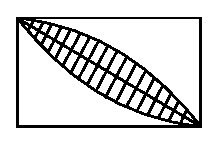
\includegraphics{figure/fig1.eps}
\end{figure}\pageoriginale

In this section we have introduced Brownian Motion corresponding to
the operator $\dfrac{1}{2}\Delta$. Later on we shall introduce a more
general diffusion process which corresponds to the operator
$\dfrac{1}{2}\sum a_{ij}\dfrac{\p^{2}}{\p x_{i}\p x_{j}}+\sum
b_{j}\dfrac{\p}{\p x_{j}}$.
\end{remark*}

